\newpage

\section{فصل نهم}

یکسری از اهداف ریسک‌هایشان مهم است که مشخص شوند و اصلاً نمی‌توان آن‌ها را در بعد
اختیاری دید. برای مثال اگر ریسک مورد نظر از نوع امنیتی باشد بایستی ریسک و راه‌حل
آن نیز مشخص شود. ولی برخی از ریسک‌ها الزام‌آور نیست و بسته به نیاز و انتخاب
مشتری می‌باشد.

همانطور که در فصل پیشین اشاره شد، در کتاب مرجع بجای استفاده از کلمه ریسک از کلمه
\lr{Obstacle} استفاده شده است.

ریسک‌ها در حقیقت مشخص می‌کنند که در وضعیت جاری هستند و به \lr{State} بعدی
نرفته‌اند. ریسک در مورد بخش بعد از \lr{Then} صحبت می‌کند. اگر ترمز قطار را
کشیدیم باید قطار شروع به توقف کند. از نوع هدف رفتاری و \lr{Achieve} می‌باشد.
\lr{Not} آن می‌شود به آن \lr{State} که باید صفر شود نرسیده است.

\subsection{متوازی الاضلاع برعکس}

برای نمایش ریسک از شکل متوازی الضلاع برعکس استفاده می‌کنیم که نشان‌دهنده
\lr{Not} هدف می‌باشد.

\begin{figure}[H]
    \centering
    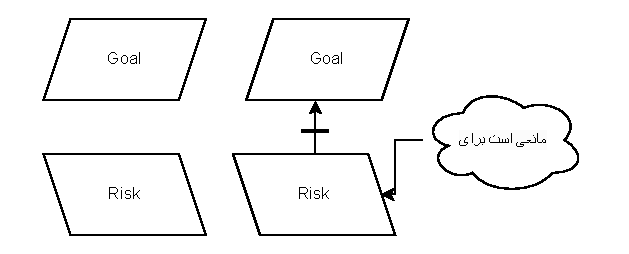
\includegraphics[width=0.9\textwidth]{assets/goal_vs_risk.drawio.pdf}
    \caption{تفاوت هدف و ریسک در نمودار ریسک}
\end{figure}

\subsection{اهدافی که باید ریسک آنها بدست آید}

۶ هدف وجود دارد که بایستی ریسکشان را بدست آوریم. چه خواسته مشتری باشد چه نباشد:

\begin{enumerate}
    \item \lr{Hazard}: از دسته اهداف \lr{Safety} می‌باشد.
    \item \lr{Threat}: از دسته اهداف امنیتی می‌باشد مانند: \lr{Disclosure,
    Corruption, DOS (Denial-of-Service), Availability, Respectively}
    \item \lr{Dissatisfaction}: از نوع در خواست‌های عوامل \lr{Satisfaction}
    می‌باشد.
    \item \lr{Misinformation}: اهداف \lr{Information}
    \item \lr{Accuracy}: ریسک ناسازگاری بین وضعیت مقادیر کنترل شونده به وسیله
    عوامل نرم‌افزاری و وضعیت تطابق تعداد موارد کنترل شده به وسیله عواملی محیطی
    است (\lr{Inaccuracy}).
    \item \lr{Unusability}: نسبت به اهداف \lr{Usability} می‌باشد.
\end{enumerate}

\begin{figure}[H]
    \centering
    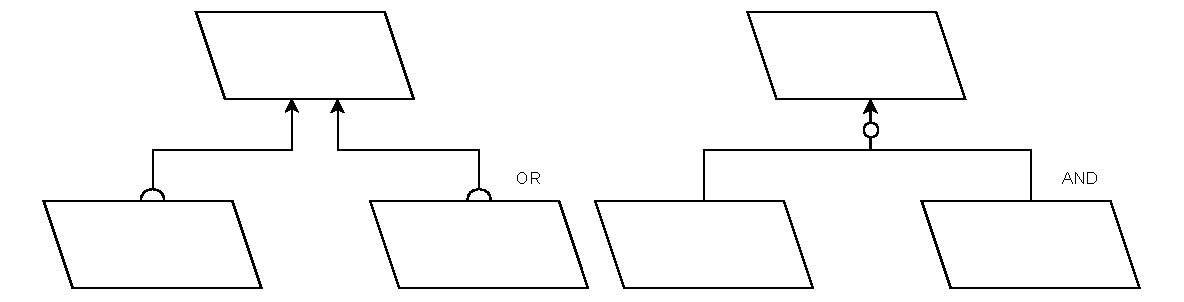
\includegraphics[width=0.9\textwidth]{assets/risk_tree_or_and_re.drawio.pdf}
    \caption{نمودار درخت ریسک}
\end{figure}

\subsection{مثال درخت ریسک تماس با آمبولانس در زمان تصادف}

\begin{figure}[H]
    \centering
    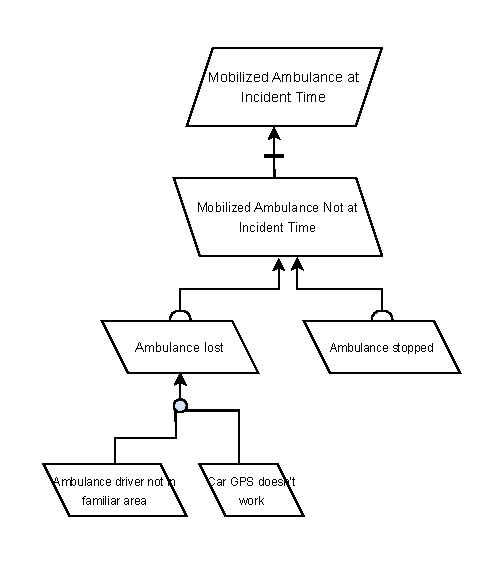
\includegraphics[width=0.6\textwidth]{assets/ambulance_risk_diagram_example.drawio.pdf}
    \caption{نمودار ریسک سناریو آمبولانس}
\end{figure}

\subsection*{نکات تکمیلی}

\begin{itemize}
    \item هر ریسکی ممکن است به درخت ختم نشود.
    \item یک ریسک می‌تواند مانعی برای رسیدن به هدف باشد.
    \item الزامات باید به یک المان در درخت هدف متصل شود.
    \item هنگام اتصال ریسک‌ها باید نسبت به آن ۶ دسته‌بندی اهداف بررسی شود. در
    حقیقت مانند یک چسب دو طرفه این کار را انجام می‌دهد.
    \item اول باید آن ۶ دسته‌بندی را حساب کنیم که مستقل نباشند.
    \item وقتی در مورد درخت ریسک صحبت می‌کنیم بایستی بچه‌های ریسک را رسم کنیم.
    \item درخت ریسک همانند درخت هدف می‌باشد با این تفاوت از اشکال هندسی خاص
    دیگری استفاده می‌کند. برای مثال برای هر ریسک از متوازی الاضلاع برعکس استفاده
    می‌کند.
    \item مقدار \lr{Criticality} از روش \lr{DDP} نسبت راه‌حل به یک یا چند ریسک،
    استفاده می‌کند.
    \item پر کردن نقاط به صورت افقی انجام می‌شود.
    \item آنقدر ریسک را می‌شکنیم که بتوانیم حاشیه را بنویسیم.
    \item اگر \lr{AND} باشد مینیموم عدد را می‌نویسیم.
    \item اگر \lr{OR} باشد ماکسیموم عدد را می‌نویسیم.
    \item در حقیقت عدد مورد نظر، همان احتمال وقوع ریسک و \lr{Criticality} رخ
    دادن ریسک است.
    \item برای نوشتن اعداد احتمال ریسک و \lr{Criticality} از \lr{Annotation}
    استفاده می‌کنیم.
    \item راه‌حل‌ها بایستی از جنس قابلیت \footnote{\lr{Feature}} باشند.
\end{itemize}

\begin{figure}[H]
    \centering
    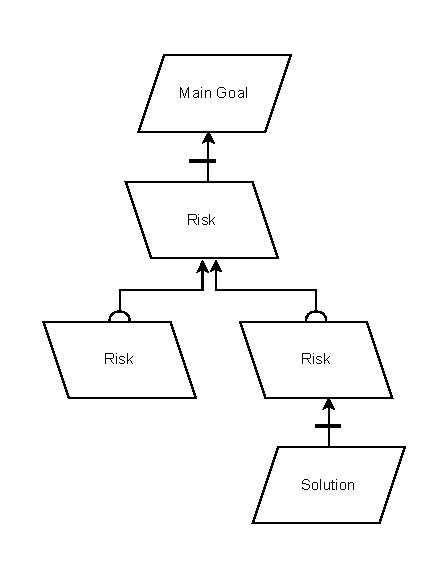
\includegraphics[width=0.5\textwidth]{assets/solution_for_risk_tree.drawio.pdf}
    \caption{نمودار درخت ریسک که یک راه‌حل را برای برطرف کردن ریسک مورد نظر
    ارائه می‌دهد.}
\end{figure}

\subsection{تاتولوژی (\lr{Tautology})}

\begin{itemize}
    \item هر چیزی که از تاتولوژی نتیجه بگیرد، \lr{AND} یا \lr{OR} آن تو نقطه تو
    پر خواهد بود.
    \item از قواعد دمورگان و ساختمان گسسته استفاده می‌کند.
    \item داخل هدف بسیار کمک کننده می‌باشد.
    % \item TODO: Learn more about -> a: reverse .... iff B: wheels turning
    \item در تاتولوژی شکست جزئیات کامل خواهیم داشت.
    \item اگر بین شروط تاتولوژی نبود یعنی تاتولوژی برای شکست این ریسک کاری از آن
    بر نمی‌آید.
    \item هر ریسک ناشناخته‌ای را می‌تواند به جزئی‌ترین بخش بشکند.
    \item ممکن است در همه جا کشش نداشته باشد.
\end{itemize}

\subsubsection{\lr{Tautology-based refinement}}

الگو‌های تاتولوژی که می‌توانند در پیدا کردن ریسک‌ها موثر باشند:

\begin{LTR}
    \begin{itemize}
        \item $NOT$(A AND B) amounts to $NOT$ A OR $NOT$ B
        \item $NOT$(if A then B) amounts to $A$ AND $NOT$ B
        \item $NOT$(A iff B) amounts to (A AND $NOT$ B) OR $(NOT$ A AND B)
        \item $NOT$(A OR B) amounts $NOT$ A and $NOT$ B
    \end{itemize}
\end{LTR}

\subsection{احتمال ریسک در اهداف \lr{Achieve}}

\begin{LTR}
    Achieve [targetCondition]: [if currentCondition then] sooner-or-later targetCondition
\end{LTR}

با $NOT$ کردن هدف ما میذتوانیم به ریشه ریسک برسیم:

\begin{LTR}
    [currentCondition and] always $NOT$ targetCondition
\end{LTR}

\subsection{ارتباط با قواعد ساختمان گسسته}

در زیر می‌توانید حضور قاعده دمورگان را برای ریسک دو هدف مشاهده کنید:

\begin{LTR}
    NOT (G1 AND G2) $\rightarrow$ (is logically equivalent to) NOT G1 OR NOT G2
\end{LTR}

\begin{figure}[H]
    \centering
    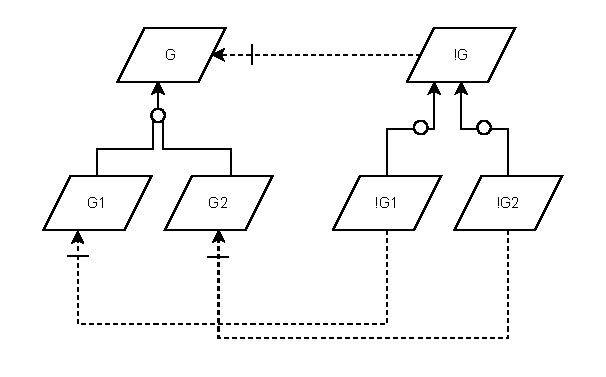
\includegraphics[width=0.6\textwidth]{assets/de-morgan.drawio.pdf}
    \caption{اعمال قاعده دمورگان در نمودار ریسک و هدف}
\end{figure}

\subsection{سناریو شرکت‌کنندگان جلسه آنلاین}

\begin{figure}[H]
    \centering
    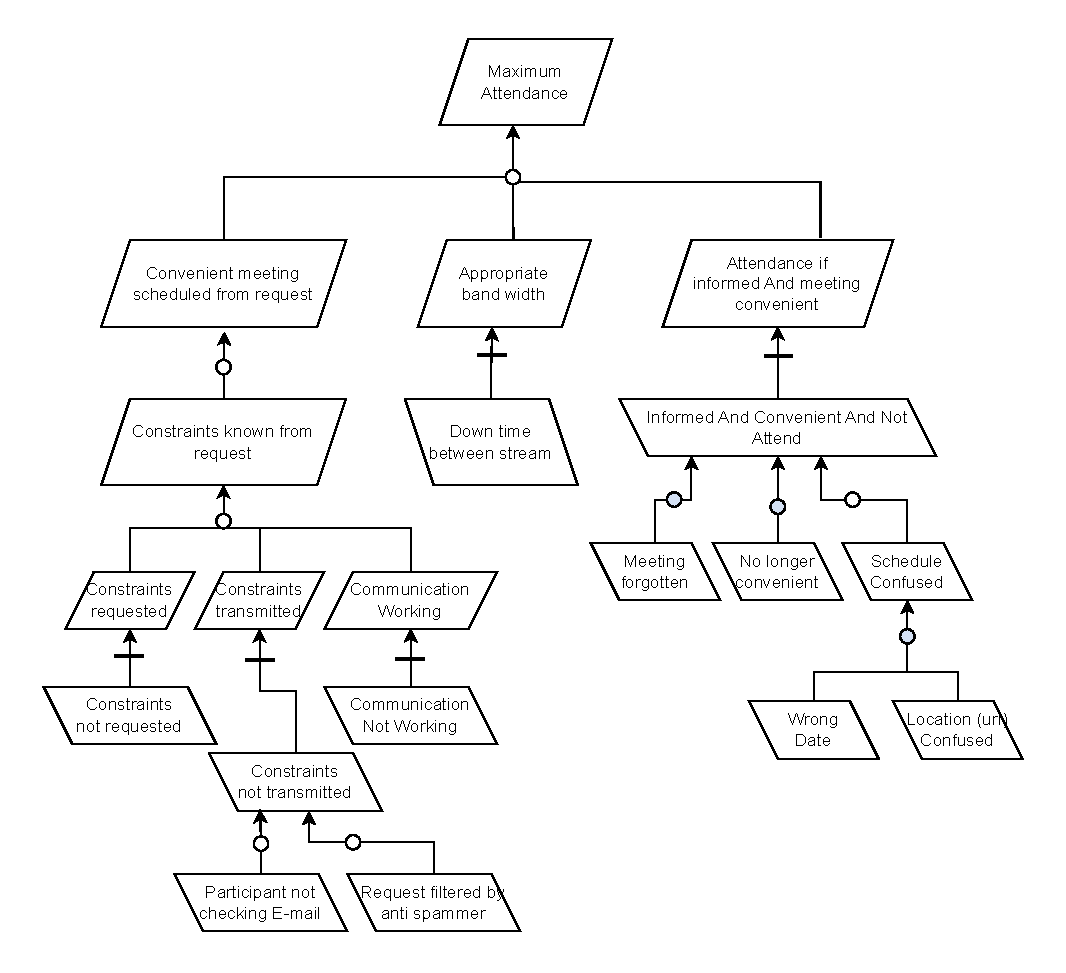
\includegraphics[width=0.8\textwidth]{assets/online_attendance.drawio.pdf}
    \caption{نمودار درخت ریسک به همراه اهداف}
\end{figure}

\subsection{شناخت شرایط لازم}

اکثر اهداف درخت از نوع رفتاری \lr{Achieve} و \lr{Maintain} هستند.

\begin{LTR}
    If a block signal is set to "stop" \textbf{then} any arriving train is
    stopped at it.
\end{LTR}

در جمله بالا ریسک اصلی بعد از \textbf{\lr{then}} می‌تواند رخ دهد:

\begin{LTR}
    A block signal is set to "stop" \textbf{and} some arriving train is
    \textbf{not} stopped at it.
\end{LTR}

\subsection{اهداف \lr{Achieve} و \lr{Maintain}}

\begin{figure}[H]
    \centering
    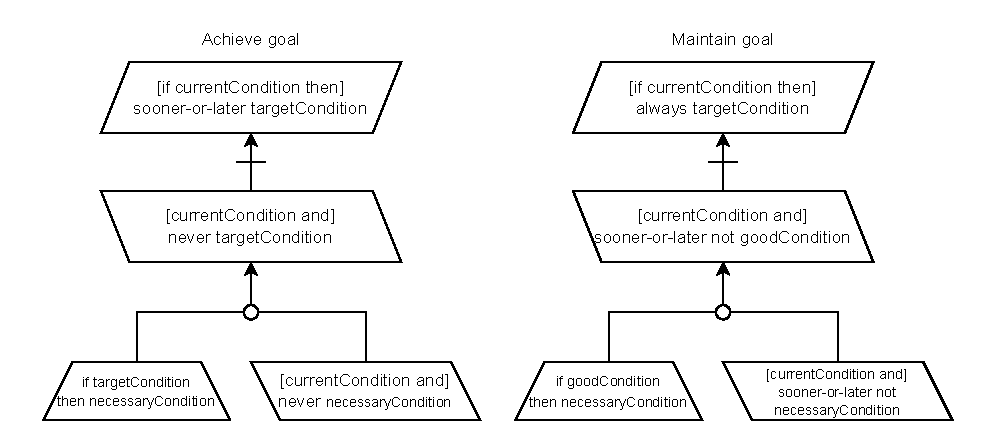
\includegraphics[width=0.8\textwidth]{assets/achieve_maintain_goal.drawio.pdf}
    \caption{تعریف ریسک در اهداف \lr{Maintain} و \lr{Achieve}}
\end{figure}